\documentclass[eng,printmode,oneside]{mgr}
\usepackage[MeX]{polski}
\usepackage[utf8]{inputenc}
\usepackage[T1]{fontenc} 
\usepackage{graphicx}
\usepackage{subfigure}
\usepackage{psfrag}
\usepackage{amsmath}
\usepackage{amsfonts}
%\usepackage{supertabular}
\usepackage{array}
\usepackage{tabularx}
\usepackage{hhline}
\usepackage{rev}
%\usepackage{framed}
\usepackage{color}
\usepackage{url}
%\usepackage[notref]{showkeys}
%\usepackage{showlabels}
\usepackage{float}
%\usepackage{tikz}
\usepackage{enumitem} 
\usepackage{graphicx}       
\usepackage{rotating}       % pakiet umożliwiający obracanie rysunków
\usepackage{subfigure}      % pakiet umożliwiający tworzenie podrysunków
\usepackage{epic}           
\usepackage{listings}       % pakiet dedykowany zrodlom programow
\usepackage{verbatim}       % pakiet dedykowany rozmaitym wydrukom tekstowym
\usepackage{amssymb}        % pakiet z rozmaitymi symbolami matematycznymi
\usepackage{amsmath}        % pakiet z rozmaitymi środowiskami matematycznymi
\usepackage[polish]{babel}  % pakiet lokalizujący dokument w języku polskim
\usepackage[OT4]{fontenc}
\usepackage[utf8]{inputenc}
\usepackage{bm}
\usepackage{gensymb}
\usepackage{booktabs}
\usepackage{epstopdf}
\usepackage{amssymb}
\usepackage[utf8]{inputenc}
\usepackage{amsmath}
\usepackage{amsfonts}
\usepackage{amssymb}
\usepackage{graphics}
\usepackage[]{algorithmic} %pseudocode
\usepackage[]{algorithm2e} %pseudocode
\usepackage{float}
\usepackage{csquotes}
\usepackage{epsfig}
%\usepackage{hyperref}
\usepackage{wrapfig} 
\reviewer{dypl}{0.2}{0.2}{0.67}
\reviewer{prof}{0.2}{0.6}{0.2}
\def\bp{\begin{review}[prof]}
\def\ep{\end{review}}
\def\bdypl{\begin{review}[dypl]}
\def\edypl{\end{review}}
\newcommand{\R}{I\!\!R} 
\newtheorem{theorem}{Twierdzenie}[section] 
\newcommand\numberthis{\addtocounter{equation}{1}\tag{\theequation}}
\newenvironment{myitemize}%
 { \begin{list}{\labelitemi}%
   {
      \setlength{\itemsep}{0mm}%
      \setlength{\topsep}{6pt}%
      \setlength{\leftmargin}{5mm}%
     \setlength{\parsep}{1mm}%
    }
  }
{\end{list}
}
\newcounter{mycount}
\newenvironment{MYenumerate}%
 {\begin{list}{\arabic{mycount}.}%
   {\usecounter{mycount}%
%      \setlength{\topsep}{12pt}%
      \setlength{\topsep}{6pt}%
      \setlength{\itemsep}{0mm}%
      \setlength{\leftmargin}{7mm}%
     \setlength{\parsep}{1mm}%
    }%
 }%
{\end{list}}
\newenvironment{todo}
{
\label{todo}
\color{red} [
}
{]
}
%%%%%%%%%chapter no new page%
\usepackage{etoolbox}
\makeatletter
\patchcmd{\chapter}{\if@openright\cleardoublepage\else\clearpage\fi}{}{}{}
\makeatother
%%%%%%%%%%%%%
\title{?}
\engtitle{?}

\author{inż. Bernard Malec}
\supervisor{Prof.\ dr hab.\ inż.\ Alicja Mazur}


\field{Automatyka i Robotyka (AIR)}
\specialisation{Robotyka (ARR)}

%\includeonly{mch0,mch1,mch2,mch3,mch4,bibl}
%\includeonly{mch3}

\begin{document}
\bibliographystyle{plabbrv} %BibTeX polski styl bibliografii 

% te ozdobniki dodaje się dopiero na końcu 
%\maketitle
\tableofcontents

\chapter{Wstęp}
\section{Cel pracy}
\section{Zawartość pracy}
\chapter{Model manipulatora mobilnego}
Manipulator mobilny to platforma mobilna z zamontowanym na niej manipulatorem. Biorąc pod uwagę typ ograniczeń nałożonych kolejno na platformę i manipulator można wydzielić 4 typy manipulatorów mobilnych:
\begin{enumerate}
\item typ (\textit{h,h}) -- platforma i manipulator związane są ograniczeniami holonomicznymi,
\item typ (\textit{nh,h}) -- na platformę nałożone są ograniczenia nieholonomiczne, natomiast na manipulator ograniczenia holonomiczne,
\item typ (\textit{nh,nh}) -- ograniczenia nałożone na platformę i manipulator są nieholonomiczne. Taki  rodzaj manipulatora mobilnego został przedstawiony w \cite{5},
\item typ (\textit{h,nh}) -- na manipulator  nałożone są ograniczenia nieholonomiczne, natomiast na platformę holonomiczne.
\end{enumerate} 

W tym rozdziale zostanie przedstawiony model manipulatora mobilnego typu (\textit{nh,h}). W szczególności w rozważanym manipulatorze platformą będzie monocykl, czyli robot mobilny klasy (2,0). Za manipulator natomiast posłuży manipulator RTR. Rozważany manipulator mobilny przedstawiono na rys \ref{ziemskii}.
\begin{figure}[H]
\centering
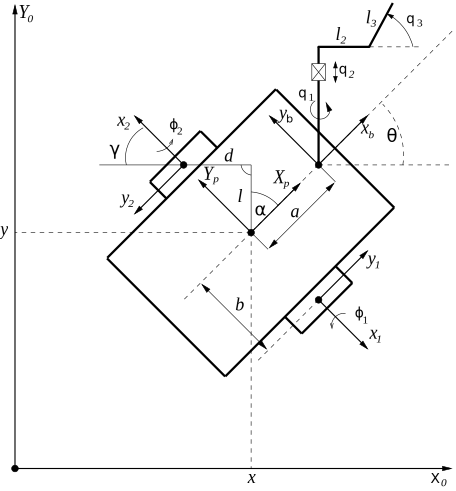
\includegraphics[width=.6\linewidth]{pics/ziemskii}
\caption{Manipulator mobilny z platformą klasy (2,0) i manipulatorem RTR}
\label{ziemskii}
\end{figure}
Przyjmijmy następujący wektor współrzędnych uogólnionych manipulatora mobilnego:
\begin{equation}
q=\left(
\begin{array}{c}
q_m\\
q_r\\
\end{array}
\right)\in R^{n+p},
\end{equation}
gdzie $q_m=(x,y,\theta, \phi_1, \phi_2)^T \in R^n$ -- wektor współrzędnych uogólnionych platformy mobilnej, $q_r=(q_1,q_2,q_3)^T \in R^p$ -- wektor współrzędnych przegubowych manipulatora. Rozmiary przestrzeni wyniosą więc $n=5$, $p=3$.
\section{Model we współrzędnych uogólnionych} \label{model1s}
Do wyprowadzenia równań manipulatora mobilnego wykorzystamy formalizm Langrange'a.\\ Lagranżjan L jest zdefiniowany jako różnica pomiędzy energią kinetyczną, a potencjalną układu
\begin{equation}
L(q,\dot{q})=T(q,\dot{q})-V(q).
\end{equation}
Równania ruchu przy braku sił działających na system są następujące
\begin{equation}
\label{lagrange}
\frac{d}{dt}\left(\frac{\partial L}{\partial\dot{q}}\right)-\frac{\partial L}{\partial q}=0.
\end{equation}
Lewą stronę równania \eqref{lagrange} można przedstawić jako
\begin{equation}
\label{lagrange2}
\frac{d}{dt}\left(\frac{\partial L}{\partial \dot{q}}\right)-\frac{\partial L}{\partial q}=Q(q)\ddot{q}+C(q,\dot{q})\dot{q}+D(q).
\end{equation}
Przy obecności sił zewnętrznych równanie \eqref{lagrange} wygląda następująco
\begin{equation}
\label{lagrange3}
Q(q)\ddot{q}+C(q,\dot{q})\dot{q}+D(q)=F_e.
\end{equation}
W naszym przypadku siły zewnętrze $F_e$ są sumą 2 składowych: $F_e=B(q)u+F_{nh}$, gdzie $B(q)u$ to uogólnione siły wejściowe(tj. wywierane na system przez elementy wykonawcze), a $F_{nh}$ to siły więzów nieholonomicznych(tj. siły zapewniające spełnienie ograniczeń nieholonomicznych). Wektor $u=\left(
\begin{array}{c}
u_m\\
u_r
\end{array}\right)\in R^{(n+p-l)}$ jest wektorem sterowań.\\ Macierz
$B(q)=\begin{bmatrix}
    B(q_m)  &0\\
    0  &I_p \\
\end{bmatrix} \in R^{(n+p)\times(n+p-l)} $ nazywana jest macierzą wejściową. \\Symbol $l$ oznacza liczbę ograniczeń nieholonomicznych.\\ Łatwo zauważyć, że jeśli obecne jest chociaż jedno ograniczenie nieholonomiczne, to macierz $B(q)$ nie jest macierzą kwadratową, przez co nie można jej odwrócić. 
\subsection{Ograniczenia nieholonomiczne}
W ninejszej pracy platformą manipulatora mobilnego jest monocykl. W założeniu ma poruszać się on bez poślizgu wzdłużnego i poprzecznego kół. Aby zapewnić spełnienie tych założeń, należy nałożyć trzy ograniczenia. Można pokazać, że jedynie dwa z nich to ograniczenia nieholonomiczne, a ostatnie można scałkować do ograniczenia holonomicznego i w rezultacie wyeliminować jedną współrzędną z $q_m$ \cite{7}. Aby jednak pokazać możliwość algorytmu w działaniu przy obecności ograniczeń holonomicznych i nieholonomicznych potraktujmy wszystkie trzy jednakowo i nie całkujmy żadnego z nich.\\
\par Przedstawmy ograniczenia w postaci Pfaffa
\begin{equation}
\label{pfaff}
A(q)\dot{q}=0,
\end{equation}
Ponieważ ograniczenia te dotyczą tylko platformy, zapiszmy $A(q)$ następująco 
\begin{equation}
A(q)=\begin{bmatrix}
   A(q_m)&0\\
\end{bmatrix}
\in R^{l\times(n+p)}.
\end{equation}
Z \cite{6} wiemy, że siła więzów nieholonomicznych równa jest $F_{nh}=A(q)^T\lambda$, gdzie $\lambda$ to wektor mnożników Lagrange'a. Równanie dynamiki wyrażone we współrzędnych uogólnionych (\ref{lagrange3}) można więc teraz zapisać jako
\begin{equation}
\label{lagrange4}
Q(q)\ddot{q}+C(q,\dot{q})\dot{q}+D(q)=B(q)u+A(q)^T\lambda .
\end{equation}
\section{Model w prędkościach pomocniczych}
Model postaci (\ref{lagrange4}) posiada pewne wady: jak wspomniano, pojawiająca się w (\ref{model1s}) macierz $B(q)$ nie daje się odwrócić z powodu obecności ograniczeń nieholonomicznych. W jawnej postaci występują również mnożniki Lagrange'a odpowiadające siłom tarcia statycznego zależnego od $u$, $q$, $\dot{q}$, $t$. Aby pozbyć się tych wad można przekształcić (\ref{lagrange4}) do modelu wyrażonego w prędkościach pomocniczych.\\
\par Zauważmy najpierw, że ograniczenia (\ref{pfaff}) wymagają, aby prędkość $\dot{q}$ należała do jądra macierzy $A(q)$. \\
Niech baza jądra $A(q_m)$ będzie zbiorem wektorów $\{g_1(q_m), g_2(q_m),..., g_{n-l}(q_m)\}$. Zapiszmy prędkość platformy $\dot{q}_m$ w następujący sposób 
\begin{equation}
\dot{q}_m=\sum_{k=1}^{n-l} g_k(q_m)\eta_k=\begin{bmatrix}
   g_1(q_m)& g_2(q_m)&...& g_{n-l}(q_m)\\
\end{bmatrix}
\left(
\begin{array}{c}
\eta_1\\
\vdots\\
\eta_{n-l}
\end{array}\right)
=G_m(q_m)\eta.
\end{equation}
Wektor $\eta$ nazywamy wektorem prędkości pomocniczych.\\
Zauważmy, że wektor prędkość całego manipulatora mobilnego można przedstawić jako 
\begin{equation}
\label{niewiem1}
\dot{q}=G(q)z,
\end{equation}
gdzie $G(q)=\begin{bmatrix}
    G_m(q_m)  &0\\
    0  &I_p \\
\end{bmatrix}\in R^{(n+p)\times(n+p-l)}$ i $z=\left(
\begin{array}{c}
\eta\\
\dot{q}_r\\
\end{array}
\right)\in R^{(n+p-l)}$ należy do jądra macierzy $A(q)$ i tym samym spełnia ograniczenia (\ref{pfaff}).
\par Możemy więc zapisać, że
\begin{equation}
\label{AG}
A(q)G(q)=0.
\end{equation}
Biorąc transpozycje (\ref{AG}) otrzymamy
\begin{equation}
\label{AG2}
G^T(q)A^T(q)=0^T.
\end{equation}
Aby wyeliminować mnożniki Lagrange'a z (\ref{lagrange4}), należy pomnożyć (\ref{lagrange4}) lewostronnie przez  $G^T$(dla czytelności pomińmy argumenty) i skorzystać z (\ref{AG2}). Otrzymamy wtedy
\begin{equation}
\label{predkoscipomoc1}
G^TQ\ddot{q}+G^TC\dot{q}+G^TD=G^TBu+G^TA^T\lambda =G^TBu.
\end{equation}
Zróżniczkujmy jeszcze (\ref{niewiem1}) po czasie
\begin{equation}
\label{niewiem2}
\ddot{q}=\dot{G}z+G\dot{z}.
\end{equation}
Po podstawieniu (\ref{niewiem1}) i (\ref{niewiem2}) do (\ref{predkoscipomoc1}), otrzymamy model w prędkościach pomocniczych:
\begin{equation}
G^TQ(\dot{G}z+G\dot{z})+G^TCGz+G^TD=G^TQG\dot{z}+G^T(Q\dot{G}+CG)z+G^TD=G^TBu,
\end{equation}
czyli
\begin{equation}
\label{modelpp}
Q^*\dot{z}+C^*z+D^*=B^*u,
\end{equation}
gdzie:
\begin{align*}
 Q^*&=G^TQG,\\
 C^*&=G^T(Q\dot{G}+CG),\\
 D^*&=G^TD,\\
 B^*&=G^TB.
\end{align*}
Równanie (\ref{modelpp}) opisuje dynamikę manipulatora mobilnego wyrażoną w prędkościach pomocniczych.\\

\chapter{Odsprzęganie wejściowo-wyjściowe dla manipulatora mobilnego}
Algorytm odsprzęgania wejściowo-wyjściowego jest wykorzystywany do sterowania manipulatorów mobilnych. Rozwiązuje on zadanie śledzenia zadanej trajektorii efektora $y_d(t)$ w przestrzeni zewnętrznej. Algorytm odpsprzęgania wejściowo-wyjściowego wymaga pełnej znajomości modelu manipulatora mobilnego.\\ 

 \noindent Istnieją dwie wersje tego algorytmu:
\begin{itemize}[noitemsep,topsep=0pt]
\item podstawowy algorytm Yamamoto i Yuna \cite{2},\cite{3}
\item algorytm z rozszerzonymi funkcjami wyjściowymi\cite{1}.
\end{itemize}\vspace{0.2cm}

Różnią się one wyborem funkcji wyjściowych $y(\cdot)$. Yamamoto i Yun założyli, że funkcje te będą zależne tylko od konfiguracji platformy $q_m$, natomiast Mazur pozwala, aby funkcje wyjścia były zależne zarówno od konfiguracji platformy $q_m$, jak i od konfiguracji manipulatora $q_r$. Rozdział ten poświęcony jest opisowi obu podejść.

\section{Podstawowy algorytm Yamamoto i Yuna}
\subsection{Specyfikacja podejścia}
Yamamoto i Yun założyli, że manipulator ma ustawić się w stałej konfiguracji o maksymalnej manipulowalności, a zadanie śledzenia zadanej trajektorii ma być realizowane jedynie poprzez ruch platformy. Podejście takie traktuje cały manipulator mobilny bardziej jako samą platformę do której przymocowany jest unieruchomiony manipulator, niż pełen system, gdzie platforma i manipulator działają równocześnie.\\
Podstawowy algorytm Yamamoto i Yuna można stosować, np. gdy manipulator ma pozostać nieruchomy.

\subsection{Wybór konfiguracji manipulatora}
Ponieważ manipulator nie uczestniczy czynnie w realizacji zadania należy ustawić go w takiej konfigurację, aby ułatwić platformie realizację zadania. Za przykładem Yamamoto i Yuna wybierzmy konfigurację maksymalizującą manipulowalność. Manipulowalność manipulatora zdefiniowana jest jako \cite{7}
\begin{equation}
\label{manipulowa}
w=\sqrt{\det(J(q_r)J^T(q_r))},
\end{equation} 
gdzie $J(q_r)$ to jakobian manipulatora. Jeśli manipulator jest nieredundantny, to manipulowalność (\ref{manipulowa}) można zredukować do
 \begin{equation}
w=|\det(J(q_r))|.
\end{equation} 
Pożądaną konfigurację  maksymalizującą manipulowalność można osiągnąć w trakcie działania algorytmu, ale mając na względzie przedstawienie algorytmu w prosty sposób założymy, że ustawił się on w tej konfiguracji wcześniej.
\subsection{Funkcje wyjścia}
Algorytm Yamamoto i Yuna wymaga, aby funkcje wyjścia były zależne jedynie od konfiguracji platformy tj. $y(q_m,\bar{q}_r)=y(q_m)$. Symbol $\bar{q}_r$ oznacza stałą konfigurację manipulatora. Wybór funkcji wyjścia należy podporządkować rodzajowi zadania, jakie należy zrealizować.
\subsection{Algorytm sterowania}
\label{YYalgster}
Przed wyprowadzeniem algorytmu Yamamoto i Yuna zlinearyzujmy dynamikę manipulatora mobilnego (\ref{modelpp}). Nie jest to krok konieczny, ale ułatwia on późniejsze obliczenia. Do linearyzacji dynamiki wykorzystamy prawo sterowania z grupy 'obliczanego momentu'
\begin{equation}
\label{comTor}
u=B^{*(-1)}[C^*z+D^*+Q^*v].
\end{equation}
Po użyciu sterowania (\ref{comTor}) do modelu (\ref{modelpp}) uzyskamy system z nowym wejściem $v$ 
\begin{equation}
\label{eq:22}
\dot{z}=\left(
\begin{array}{c}
\dot{\eta}\\
\ddot{q}_r\\
\end{array}
\right)=v.
\end{equation}
Mając liniowy model (\ref{eq:22}) wyprowadźmy algorytm Yamamoto i Yuna.\\

\par Algorytm Yamamoto i Yuna realizowany jest dzięki zastosowaniu do modelu (\ref{eq:22}) dwóch pętli sprzężenia zwrotnego.\\
\par Pierwsza pętla - pętla wewnętrzna - przekształca układ do postaci liniowej typu "podwójny integrator". Druga pętla - zewnętrzna - zapewnia realizację zadania tj. śledzenia trajektori w uzyskanym układzie liniowym.\\
\par Prawo sterowania pierwszej pętli wyprowadza się w następujący sposób: najpierw zróżniczkujmy $y(q_m)$ dwukrotnie po czasie
\begin{equation}
\label{ydot}
\dot{y}(q_m)=\frac{\partial y(q_m)}{\partial q_m}\dot{q}_m=\frac{\partial y(q_m)}{\partial q_m}G_m(q_m)\eta=\Phi_m(q_m)\eta,
\end{equation}
\begin{equation}
\label{ypp}
\ddot{y}(q_m,\dot{q}_m)=\dot{\Phi}_m(q_m,\dot{q}_m)\eta+\Phi_m(q_m) \dot{\eta}=\dot{\Phi}_m(q_m,\dot{q}_m)\eta+\Phi_m(q_m) v_m.
\end{equation} 
Macierz $\Phi_m(q_m)$ jest równa
\[
\Phi_m(q_m)= \frac{\partial y(q_m)}{\partial q_m}G_m(q_m).
\]\\
Łatwo sprawdzić, że przy użyciu następującego prawa sterowania
\begin{equation}
\label{eq:petla22}
v=\left(
\begin{array}{c}
v_m\\
0\\
\end{array}
\right),
\end{equation}
\begin{equation}
v_m=\Phi_m^{-1}(q_m)[-\dot{\Phi}_m(q_m) \eta+\zeta].
\end{equation}
do równania (\ref{ypp}) otrzymamy 
\begin{equation}
\label{testtssts}
\ddot{y}=\zeta.
\end{equation} 

Wynikowy układ liniowy (\ref{testtssts}) steruje się przy użyciu drugiej pętli. Można ją zrealizować, na przykład, jako regulator PD z korekcją:
\begin{equation}
\label{PD}
\zeta=\ddot{y}_d(t)-K_d\dot{e}(t)-K_pe(t),
\end{equation}
gdzie $\ddot{y}_d(t)$ - druga pochodna zadanej funkcji wejściowej,\\ $e(t)=y_d(t)-y(t)$, $\dot{e}(t)=\dot{y}_d(t)-\dot{y}(t)$  błąd położenia i jego pochodna,\\ $K_d>0$, $K_p>0$ - nastawy regulacji.
\paragraph{Warunki działania algorytmu}
\par Ponieważ algorytm wykorzystuje odwrotność macierzy $\Phi_m$ należy  zapewnić, aby
\begin{equation}
\det(\Phi_m(q_m))\neq0
\end{equation}

\subsection{Badania symulacyjne}\label{YYsim}
Rozważany monocykl posiada dwa wejścia (sterowania obu kół), można więc odsprząc dwie współrzędne efektora. Odsprzęgnijmy współrzędne $x$ i $y$ efektora w podstawowym układzie odniesienia ($X_0$,$Y_0$).
Funkcja wyjściowa $y(q_m,\bar{q}_r)=y(q_m)$ dla nieruchomego chwytaka, a więc ustalonych $q_1$, $q_2$, $q_3$ przyjmie wtedy postać
\begin{center}
$y(q_m)=\left(
\begin{array}{c}
    y_1(q_m) \\
    y_2(q_m)\\
\end{array}
\right)=
\left(
\begin{array}{c}
    x + ac_0 + l_2c_{01} + l_3c_{01}c_3 \\
    y + as_0 + l_2s_{01} + l_3s_{01}c_3\\
\end{array}
\right).$
\end{center}
Jakobian manipulatora będzie wtedy równy 
\begin{equation}
J(\bar{q}_r)=
\left(
\begin{array}{c}
   \dfrac{\partial y_1(q_m,\bar{q}_r)}{\partial \bar{q}_r}  \\\\
      \dfrac{\partial y_2(q_m,\bar{q}_r)}{\partial \bar{q}_r}  \\
\end{array}
\right)=\begin{bmatrix}
    -s_1(l_2+l_3c_3)  &0&-c_1s_3l_3\\
    c_1(l_2+l_3c_3)  &0&-s_1s_3l_3\\
\end{bmatrix},
\end{equation} 
w związku z czym manipulowalność (\ref{manipulowa}) dana będzie wzorem
\begin{equation}
w=|s_3||(l_2+c_3l_3)|l_3.
\end{equation} 
Pojawiające się symbole oznaczają: $c_0=\cos(\theta)$, $c_1=\cos(q_1)$, $c_3=\cos(q_3)$, $s_0=\sin(\theta)$, $s_1=\sin(q_1)$, $s_3=\sin(q_3)$, $c_{01}=\cos(\theta+q_1)$, $s_{01}=\sin(\theta+q_1)$.\\
Parametry geometryczne ustalono jako $l_2=0.3$m, $l_3=0.2$m, $a=0.2$m. Maksymalną manipulowalność osiągniemy dla $q_3=1.1314$ i dowolnych  $q_1$ i $q_2$.\\

Do symulacji wybrano więc następujące konfiguracje początkowe platformy i manipulatora 
$$q(0)=
\left(
\begin{array}{c}
x(0)\\
y(0)\\
\theta(0)\\
\phi_1(0)\\
\phi_2(0)\\
q_1(0)\\
q_2(0)\\
q_3(0)\\
\end{array}
\right)=\left(
\begin{array}{c}
0\\
0\\
0\\
0\\
0\\
0\\
0.5\\
1.1314\\
\end{array}
\right)$$.\\ 
Przyjęto zerowe prędkości początkowe $\dot{q}(0)$.

Funkcje wyjściowe w chwili $0$ były następujące
\begin{center}
$y(q_m(0))=
\left(
\begin{array}{c}
    0.5851 \\
     0 \\
     
      \end{array}
\right).$
\end{center}
Wektor pochodnych $\dot{y}$ w chwili $0$ równy był zeru.\\
Wybrano  następujące trajektorie zadane $y_d(t)$ 
\begin{center}
$y_d(t)=
\left(
\begin{array}{c}
    2t\\
    -0.3\cos{(2t)}\\
\end{array}
\right).$
\end{center}
Błąd początkowy $e(t)=y_d(t)-y(t)$ i jego pochodna były równe
\begin{center}
$e(0)=
\left(
\begin{array}{c}
   -0.5851\\
    -0.3\\
   \end{array}
\right), \hspace{1.5cm}
\dot{e}(0)=
\left(
\begin{array}{c}
    2\\
    0\\
    \end{array}
\right).$
\end{center}
Do sterowania układem liniowym użyto regulatora PD z korekcją (\ref{PD}) z nastawami $K_d=4$, $K_p=2$.
W badaniach wykorzystano środowisko Matlab/Simulink. \\
Przebiegi błędów śledzenia trajektorii chwytaka pokazano na rys. \ref{fig:ZPe}
\begin{figure}[H]
\centering
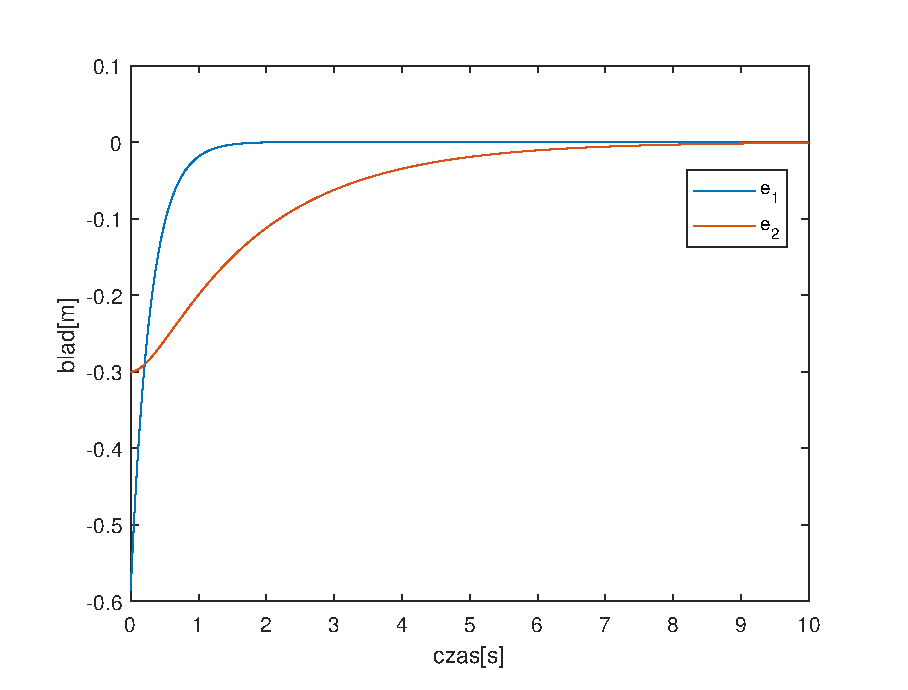
\includegraphics[width=.85\linewidth]{pics/ZPe}
\caption{Przebiegi błędów śledzenia trajektorii chwytaka}
\label{fig:ZPe}
\end{figure}

Przebiegi konfiguracji bazy i manipulatora pokazano na rys. \ref{fig:ZPq}
\begin{figure}[H]
\centering 
\begin{minipage}{.5\textwidth}
  	\centering
  	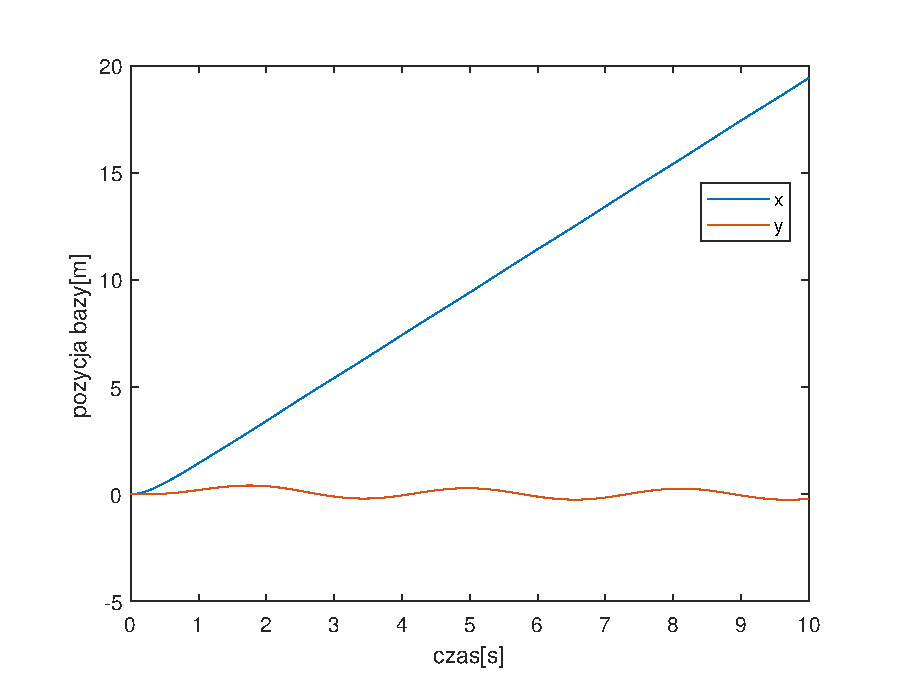
\includegraphics[width=.99\linewidth]{pics/ZPx}
  	
\end{minipage}%
\begin{minipage}{.5\textwidth}
 	\centering
    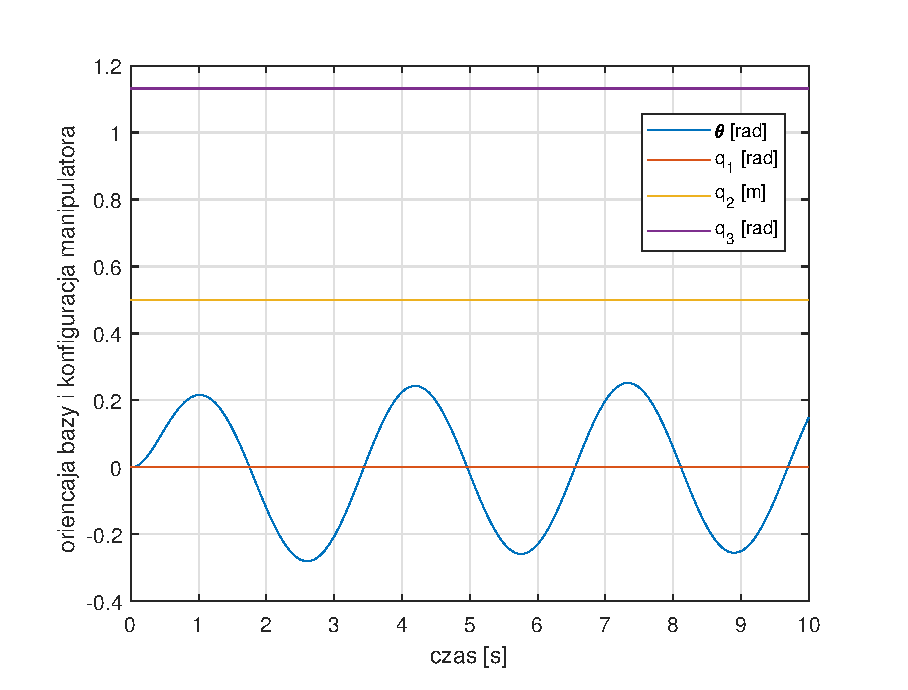
\includegraphics[width=.99\linewidth]{pics/ZPq}
\end{minipage}%
\caption{Przebiegi konfiguracji bazy i manipulatora}
\label{fig:ZPq}
\end{figure}


\begin{figure}[H]
\centering
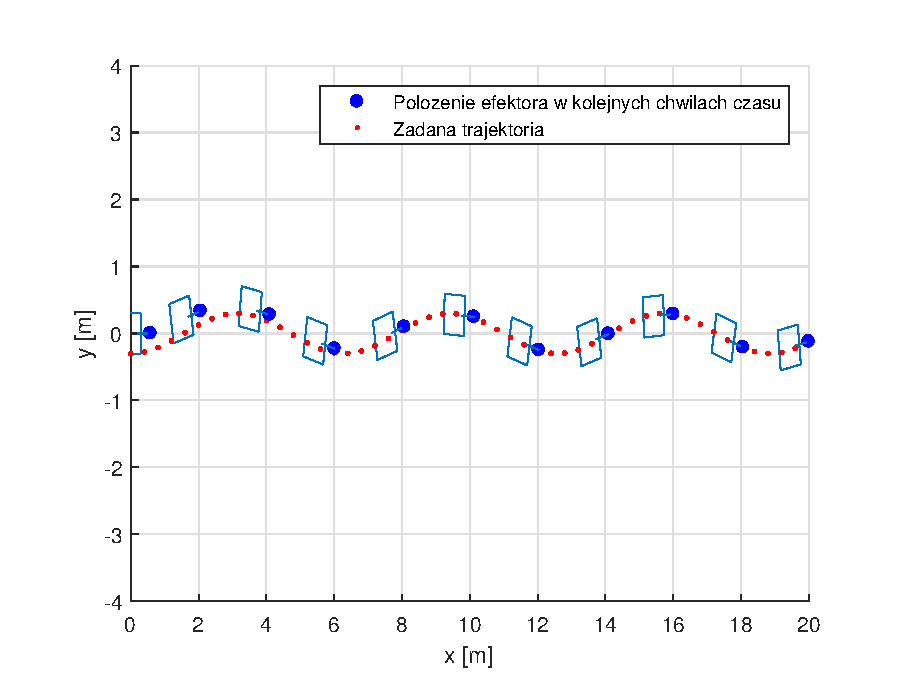
\includegraphics[width=.85\linewidth]{pics/ZPdrawingXY}
\caption{Pozycja robota w kolejnych chwilach czasu -- widok na płaszczyznę XY}
\label{ZPXY}
\end{figure}

\begin{figure}[H]
\centering
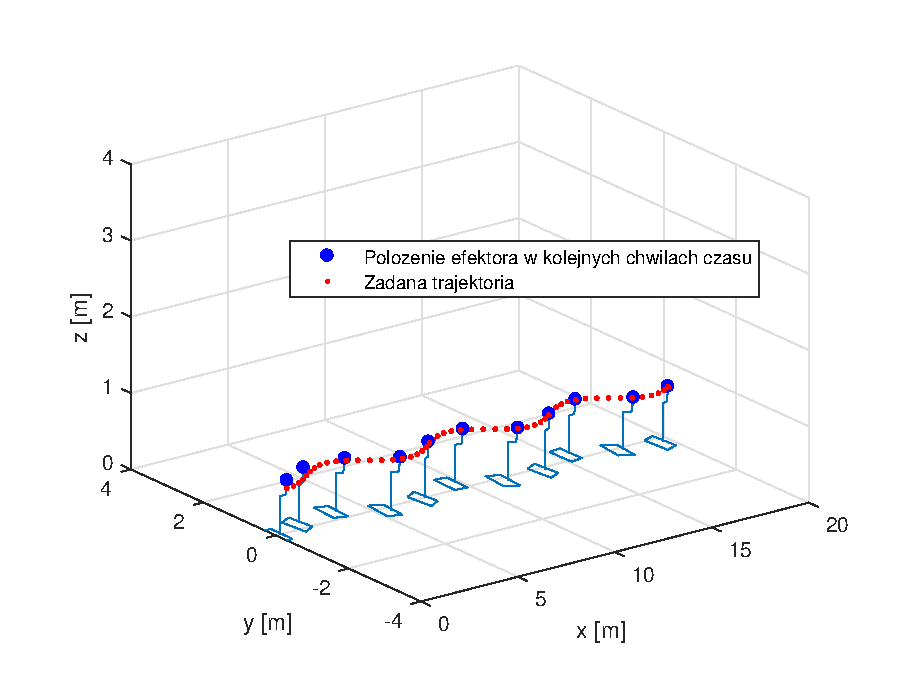
\includegraphics[width=.85\linewidth]{pics/ZPdrawingXYZ}
\caption{Pozycja robota w kolejnych chwilach czasu -- widok 3D}
\label{ZPXYZ}
\end{figure}

\section{Algorytm z rozszerzonymi funkcjami wyjściowymi}
\subsection{Specyfikacja podejścia}
Odmiennie od założeń Yamamoto i Yuna rozszerzony algorytm nie wymaga bezruchu manipulatora. Dzięki temu platforma i manipulator mogą działać równolegle w sposób skoordynowany. Sterowanie platformy nie odbywa się w sposób bezpośredni.\\
Algorytm ten stosować można nawet wówczas, gdy np. sterowanie bazą jest niemożliwe(np. w przypadku robota free-floating).
\subsection{Funkcje wyjścia}
Funkcja wyjściowa zależy teraz od konfiguracji całego robota tj. zarówno od platformy, jak i manipulatora. Przyjmuje ona postać\cite{1}:
\begin{equation}
y(q)=\left(
\begin{array}{c}
y_1(q_m,q_r)\\
y_2(q_r)\\
\end{array}
\right),
\end{equation}
gdzie $y_1(q_m,q_r)$ jest wektorem wybranych współrzędnych efektora w podstawowym układzie odniesienia ($X_0$,$Y_0$), a $y_2(q_r)$ to wektor wybranych współrzędnych efektora w lokalnym układzie odniesienia ($X_P$,$Y_P$) związanym ze środkiem masy platformy.\\
\par Liczba współrzędnych efektora w układzie ($X_0$,$Y_0$), które można odpsprząc zależy od liczby sterowań platformą. W przypadku platformy klasy $(2,0)$ możemy śledzić dwie współrzędne.\\
\subsection{Algorytm sterowania}
Przed wyprowadzeniem algorytmu odsprzęgania wejściowo-wyjściowego dla manipulatora mobilnego, zlinearyzujmy jego dynamikę (\ref{modelpp}) przy użyciu prawa sterowania z grupy 'obliczanego momentu'. Tak jak wspomniano poprzednio nie jest to krok konieczny, ale zastosujemy go w celu ułatwienia późniejszych obliczeń. Prawo sterowania linearyzujące dynamikę ma następującą postać
\begin{equation}
\label{eq:petla11}
u=B^{*-1}[C^*z+D^*+Q^*v].
\end{equation}
Po użyciu sterowania (\ref{eq:petla11}) do modelu dynamiki (\ref{modelpp}) uzyskamy system z nowym wejściem $v$
\begin{equation}
\label{eq:v2}
\dot{z}=v.
\end{equation}
\par Identycznie jak w przypadku algorytmu podstawowego, algorytm z rozszerzonymi funkcjami wyjściowymi złożony jest z dwóch pętli sprzeżenia zwrotnego\cite{1}
\begin{itemize}[noitemsep,topsep=0pt]
\item wewnętrznej pętli linearyzującej transformację wejście-wyjście
\item zewnętrznej pętli sterującej zlinearyzowanym układem
\end{itemize}
Prawo pętli wewnętrznej wyprowadzimy analogicznej jak w \ref{YYalgster}\\
Obliczmy pochodną funkcji wyjściowej $y(q)$ po czasie
\begin{equation}
\dot{y}(q)=
\left(
\begin{array}{c}
    \frac{\partial y_1}{\partial q_m} \dot{q}_m  + \frac{\partial y_1}{\partial q_r} \dot{q}_r \\
     \frac{\partial y_2}{\partial q_r} \dot{q}_r\\
\end{array}
\right)=
\begin{bmatrix}
    \frac{\partial y_1}{\partial q_m} G_m(q_m)     & \frac{\partial y_1}{\partial q_r}  \\
    0       & \frac{\partial y_2}{\partial q_r} \\
\end{bmatrix}
\left(
\begin{array}{c}
\eta\\
\dot{q}_r\\
\end{array}
\right)=\Phi(q)z,
\end{equation} 
\[
\Phi(q)=
\begin{bmatrix}
    \frac{\partial y_1}{\partial q_m} G_m(q_m)      & \frac{\partial y_1}{\partial q_r}  \\
    0       & \frac{\partial y_2}{\partial q_r} \\
\end{bmatrix}=
\begin{bmatrix}
    \Phi_m       & \Phi_{mr} \\
    0       & \Phi_r  \\
\end{bmatrix}.
\]
Ponownie zróżniczkujmy $\dot{y}(q)$ po czasie
\begin{equation}
\label{eq:edwfwsefef}
\ddot{y}(q,\dot{q})=\dot{\Phi}(q,\dot{q})z+\Phi(q) \dot{z}=\dot{\Phi}(q,\dot{q})z+\Phi(q) v.
\end{equation} 

Aby zapewnić linearyzację wejściowo-wyjściową układu (\ref{eq:edwfwsefef}) należy więc użyć następującej pętli wewnętrznej
\begin{equation}
v=\Phi^{-1}(q)[-\dot{\Phi}(q,\dot{q}) z+\zeta].
\end{equation}
Po zastosowaniu pierwszej pętli otrzymamy funkcję wyjściową o liniowej postaci
\begin{equation}
\ddot{y}(q,\dot{q})=\zeta.
\end{equation}
Otrzymaliśmy system identyczny jak ten po zastosowaniu algorytmu Yamamoto i Yuna tj. układ liniowy typu "podwójny integrator". Jego sterowaniem zajmuje się pętla zewnętrzna, którą również można zrealizować jako regulator PD z korekcją(\ref{PD}).
\paragraph{Warunki działania algorytmu} Tak jak w przypadku podstawowego algorytmu Yamamoto i Yuna należy zapewnić odwracalość macierzy $\Phi$. Warunek taki trzeba spełnić aby algorytm funkcjonował. Ma on następującą postać
\begin{equation}
\text{det}(\Phi)=\text{det}(\Phi_m)\text{det}(\Phi_r)\neq0
\end{equation}
\subsection{Badania symulacyjne}
Rozważany monocykl posiada dwa wejścia (sterowania obu kół), można więc odsprząc dwie współrzędne efektora.\\
Podczas badań odsprzęgnięto współrzędne $x$ i $y$ efektora w podstawowym układzie odniesienia ($X_0$,$Y_0$). Funkcja wyjścia $y_1(q_m,q_r)$ ma postać\\
\begin{center}
$y_1(q_m,q_r)=
\left(
\begin{array}{c}
    x + ac_0 + l_2c_{01} + l_3c_{01}c_3 \\
    y + as_0 + l_2s_{01} + l_3s_{01}c_3\\
\end{array}
\right).$
\end{center}
Funkcja $y_2(q_r)$ to wektor współrzędnych $x$, $y$ i $z$ efektora w układzie środka masy platformy ($X_P$,$Y_P$)\\
\begin{center}
$y_2(q_r)=
\left(
\begin{array}{c}
     a + l_2c_{1} + l_3c_{1}c_3 \\
     l_2s_{1} + l_3s_{1}c_3\\
     s_3l_3+q_2
\end{array}
\right).$
\end{center}
Ponownie, symbole oznaczają: $c_0=\cos(\theta)$, $c_1=\cos(q_1)$, $c_3=\cos(q_3)$, $s_0=\sin(\theta)$, $s_1=\sin(q_1)$, $s_3=\sin(q_3)$, $c_{01}=\cos(\theta+q_1)$, $s_{01}=\sin(\theta+q_1)$.\\
Parametry geometryczne ustalono jako: $l_2=0.3$m, $l_3=0.2$m, $a=0.2$m.\\
Początkowe położenie platformy było równe $q_m(0)=(x(0),y(0),\theta(0),\phi_1(0),\phi_2(0))=(0,0,0,0,0)$, a początkowa konfiguracja manipulatora była równa $q_r(0)=(q_1(0),q_2(0),q_3(0))=(\frac{\pi}{2},0.2,-\frac{\pi}{2})$.\\
Prędkości początkowe $\dot{q}(0)$ były równe zeru.  \\
Funkcje wyjściowe miały następujące wartości początkowe 
\begin{center}
$y(q_m(0),q_r(0))=
\left(
\begin{array}{c}
    0.2 \\
     0.3 \\
      0.2 \\
     0.3 \\
     0 \\
\end{array}
\right).$
\end{center}
Wektor pochodnych $\dot{y}$ był zerowy.\\
Wybrano następujące trajektorie zadane $y_d(t)$ 
\begin{center}
$y_d(t)=
\left(
\begin{array}{c}
    2t\\
    -0.3\cos{(2t)}\\
    0.5\\
    -0.3\\
    0.2\\
\end{array}
\right).$
\end{center}
Błąd początkowy $e(t)=y_d(t)-y(t)$ i jego pochodna były równe
\begin{center}
$e(0)=
\left(
\begin{array}{c}
   -0.2\\
    -0.6\\
    0.3\\
    -0.6\\
    0.2\\
\end{array}
\right), \hspace{1.5cm}
\dot{e}(0)=
\left(
\begin{array}{c}
    2\\
    0\\
    0\\
    0\\
    0\\
\end{array}
\right).$
\end{center}
Do sterowania układem liniowym użyto regulator PD z korektą (\ref{PD}) z nastawami $K_d=4$, $K_p=2$.
W badaniach wykorzystano środowisko Matlab/Simulink. \\
Przebiegi błędów śledzenia trajektorii chwytaka pokazano na rys. \ref{ZRe}

\begin{figure}[H]
\centering
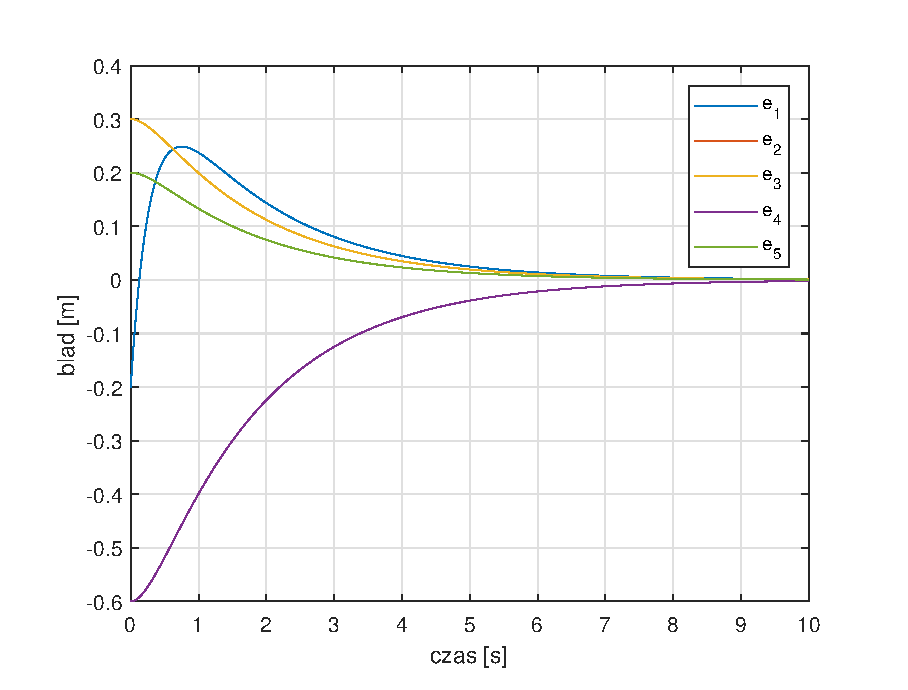
\includegraphics[width=.8\linewidth]{pics/ZRe}
\caption{Przebieg błędów śledzenia trajektorii chwytaka}
\label{ZRe}
\end{figure}

Przebiegi konfiguracji bazy i manipulatora pokazano na rys. \ref{ZRq}
\begin{figure}[H]
\centering 
\begin{minipage}{.5\textwidth}
  	\centering
  	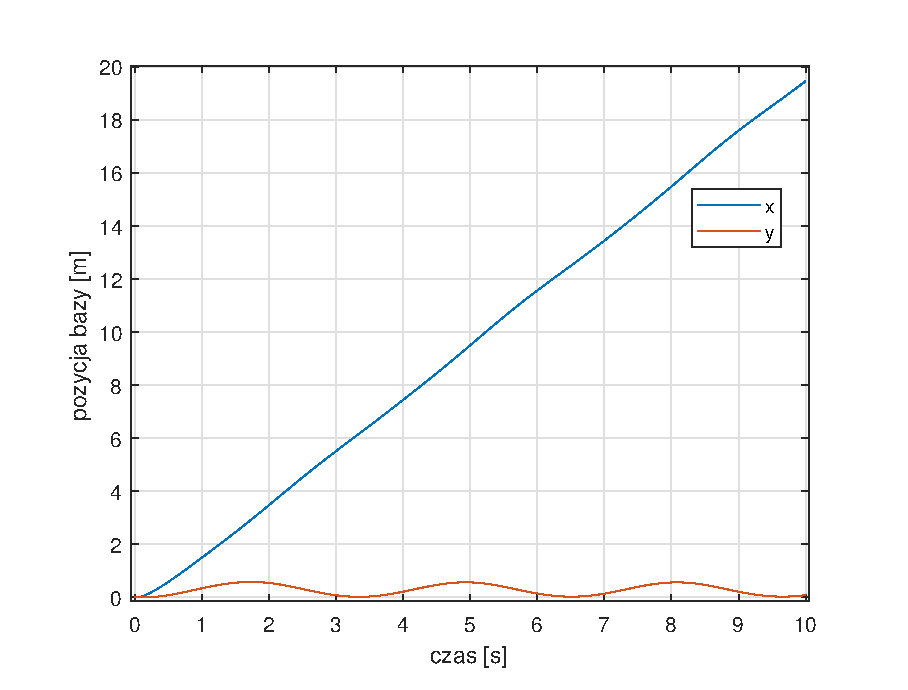
\includegraphics[width=.99\linewidth]{pics/ZRx}
\end{minipage}%
\begin{minipage}{.5\textwidth}
 	\centering
    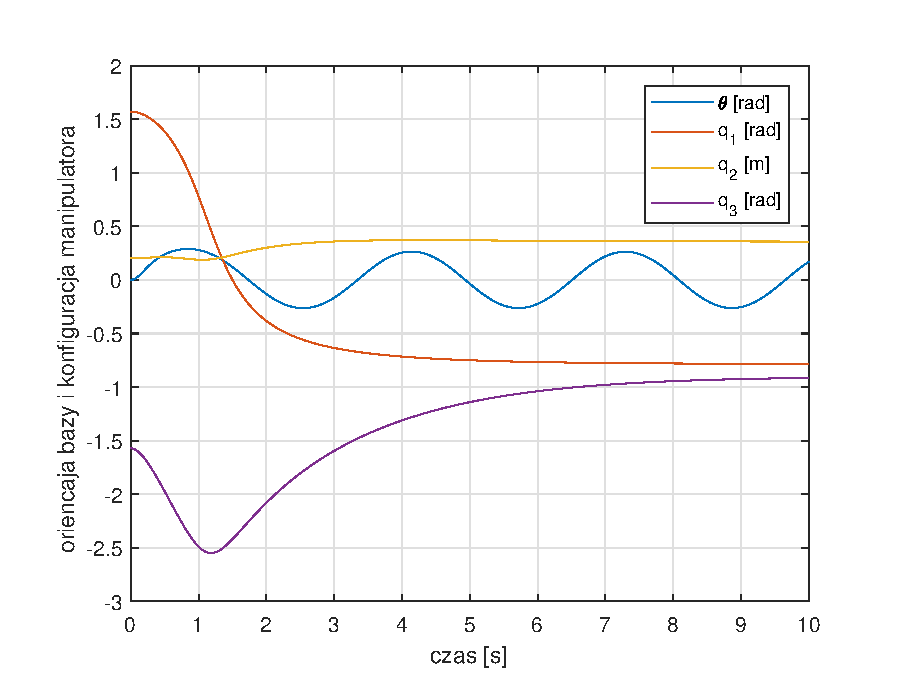
\includegraphics[width=.99\linewidth]{pics/ZRq}
\end{minipage}%
\caption{Przebieg konfiguracji bazy i manipulatora}
\label{ZRq}
\end{figure}


\begin{figure}[H]
\centering
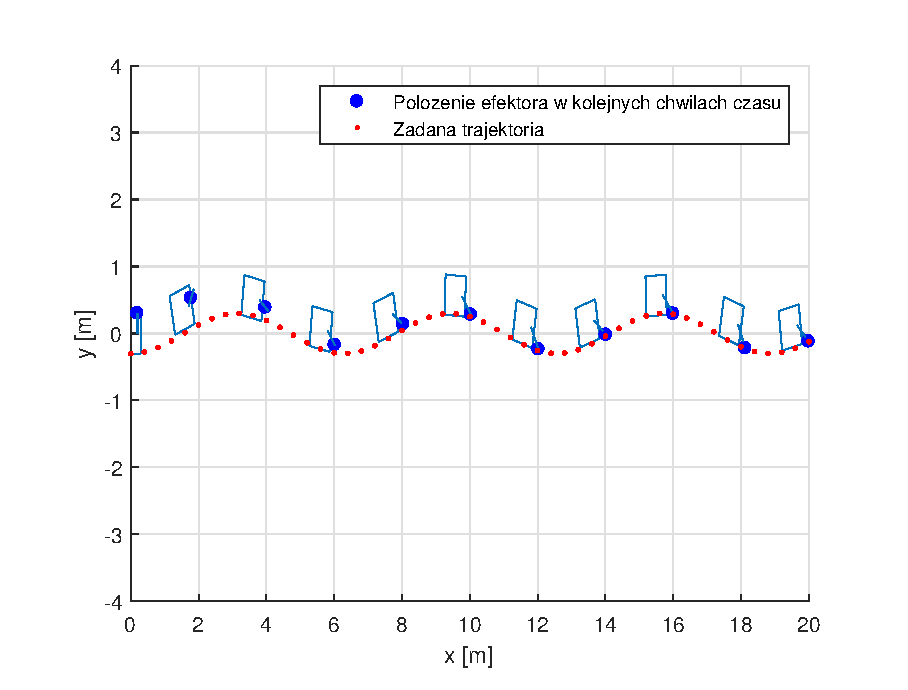
\includegraphics[width=.85\linewidth]{pics/ZRdrawingXY}
\caption{Pozycja robota w kolejnych chwilach czasu -- widok na płaszczyznę XY}
\label{ZRXY}
\end{figure}

\begin{figure}[H]
\centering
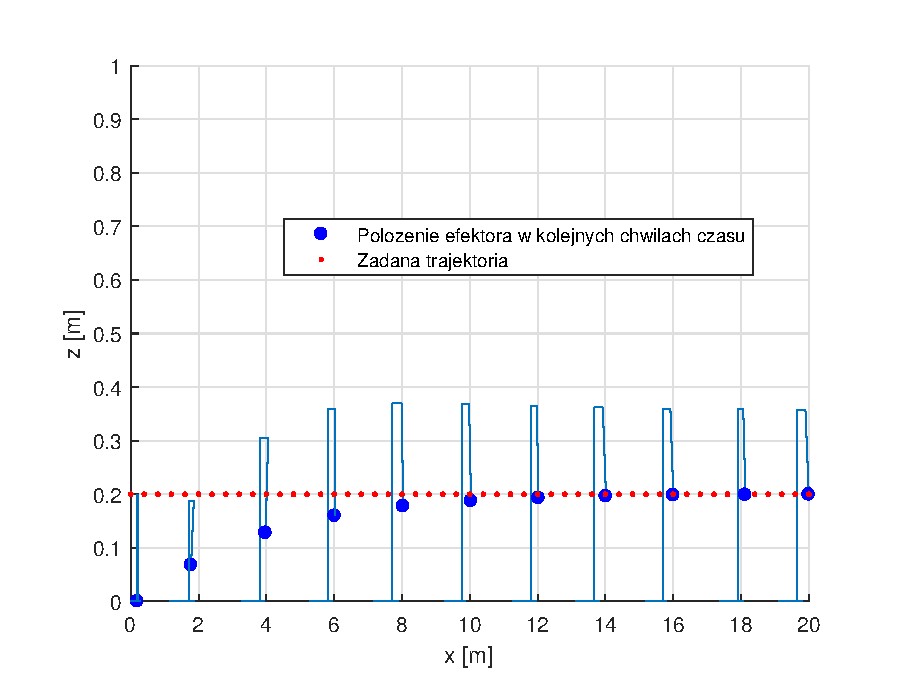
\includegraphics[width=.85\linewidth]{pics/ZRdrawingXZ}
\caption{Pozycja robota w kolejnych chwilach czasu -- widok na płaszczyznę XZ}
\label{ZRXZ}
\end{figure}

\begin{figure}[H]
\centering
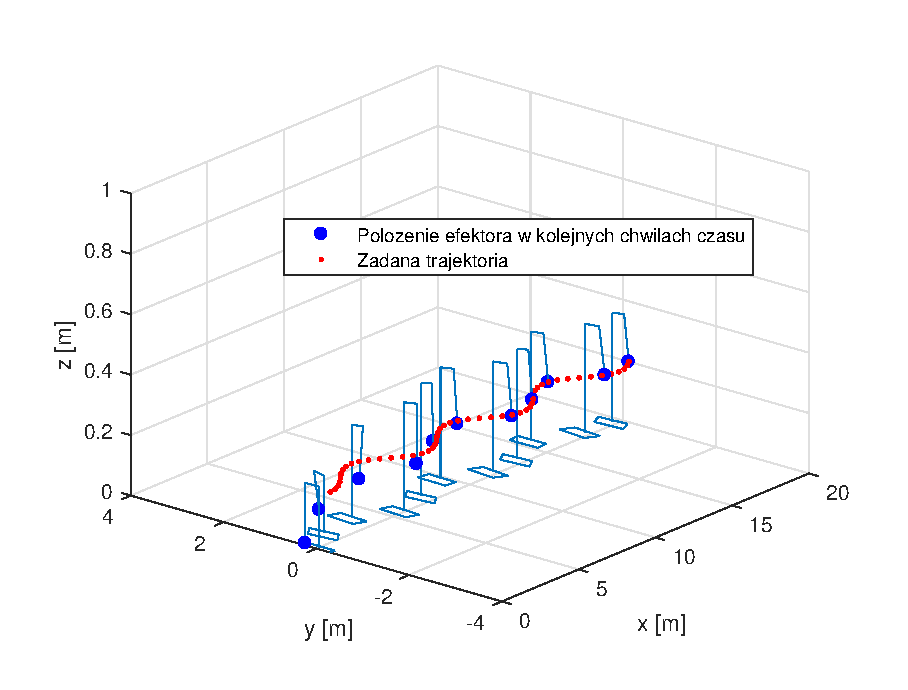
\includegraphics[width=.85\linewidth]{pics/ZRdrawingXYZ}
\caption{Pozycja robota w kolejnych chwilach czasu -- widok 3D}
\label{ZRXYZ}
\end{figure}



\chapter{Model satelity typu free-floating}
\section{Model we współrzędnych uogólnionych}
Robot free-floating z manipulatorem to nienapędzana platforma (baza) z zamontowanym na niej napędzanym manipulatorem. Robot taki znajduje się w przestrzeni kosmicznej w stanie mikrograwitacji (nieważkości).
\par W rozważanym robocie platformą będzie jednolita prostokątna płyta, a za manipulator posłuży manipulator RR. Rozważanego robota free-floating z manipulatorem przedstawiono na rys \ref{FF}. \par Robot taki jest użyteczny ze względów praktycznych. Do badań eksperymentalnych bowiem, można wykorzystać płaską granitową płytę, po której baza może ślizgać się bez tarcia. %, a siły grawitacji nie mają wpływu na dynamikę.
Dzięki temu testy można przeprowadzać na Ziemi, a nie w warunkach mikrograwitacji.
\begin{figure}[H]
\centering
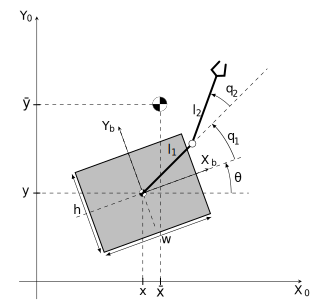
\includegraphics[width=.6\linewidth]{pics/FF}
\caption{Robot free-floating z manipulatorem}
\label{FF}
\end{figure}

\par Do wyprowadzenia modelu we współrzędnych uogólnionych weźmy następujące współrzędne
\begin{equation}
q=\left(
\begin{array}{c}
q_b\\
q_r\\
\end{array}
\right),
\end{equation}
gdzie $q_b=(x,y,\theta)^T$ -- wektor współrzędnych uogólnionych bazy, $q_r=(q_1,q_2)^T$ -- wektor współrzędnych przegubowych manipulatora. 
\par Równania dynamiki we współrzędnych uogólnionych takiego robota można, ponownie korzystając z formalizmu Langrange'a, zapisać jako\\
\begin{equation}
\label{wrsdad}
H(q)\ddot{q}+C(q,\dot{q})\dot{q}=
\left(
\begin{array}{c}
0\\
u\\
\end{array}
\right).
\end{equation}\\
Brak wektora sił potencjalncyh $D(q)$ wynika z braku grawitacji. \par Sterowanie $u$ pojawia się tylko w dolnej części równania dynamiki (\ref{wrsdad}), ponieważ dotyczy jedynie manipulatora, jako że baza jest nienapędzana (free-floating).

%\end{equation}\\
\section{Model we współrzędnych barycentrycznych}
Jeśli środek masy robota free-floating z manipulatorem ma pozostać nieruchomy (lub poruszać się ze stałą prędkością), konieczne jest zamodelowanie dynamiki we współrzędnych barycentrycznych.\\
\par Położenie środka masy robota free-floating z manipulatorem można wyliczyć z definicji jako
\begin{equation}
\left(\sum\limits^w_{i=1}m_i\right)\phi_b=\sum\limits^w_{i=1}m_ir_i,
\end{equation}
gdzie $r_i$ to środek masy $i$-tego członu robota w podstawowym układzie współrzędnych, a  $m_i$ to masa $i$-tego członu. Z kolei $w$ to liczba członów robota. W naszym przypadku $w$ wynosi trzy, robot posiada bowiem jedną bazę i dwa ramiona.\\
$\phi_b$ to współrzędne barycentryczne układu, czyli
\begin{equation}
\label{baro}
\phi_b=
\left(
\begin{array}{c}
\bar{x}\\
\bar{y}\\
\theta\\
\end{array}
\right)=
\frac{\sum\limits^w_{i=1}m_ir_i}{\sum\limits^w_{i=1}m_i}.
\end{equation}
Kompletne współrzędne barycentryczne satelity wraz z manipulatorem $\phi$ mają postać
\begin{equation}
\phi=
\left(
\begin{array}{c}
\phi_b\\
q_r\\
\end{array}
\right).
\end{equation}
Model we współrzędnych barycentrycznych można więc wyrazić jako
\begin{equation}
\bar{H}\ddot{\phi}+\bar{C}\dot{\phi}
=
\left(
\begin{array}{c}
0\\
u\\
\end{array}
\right),
\end{equation}

Macierze $\bar{H}$ i $\bar{C}$ uzyskuje się przez przeliczenie energii kinetycznej do układu współrzędnych barycentrycznych i wykorzystanie formalizmu Lagrange'a dla nowej energii kinetycznej.\\

\chapter{Odsprzęganie wejściowo-wyjściowe dla robota free-floating z manipulatorem}

Ponieważ baza robota free-floating z manipulatorem nie jest napędzana, do odsprzęgania wejściowo-wyjściowego nie można zastosować podstawowego algorytmu Yamamoto i Yuna. Do realizacji zadania śledzenia trajektorii w przestrzeni zadaniowej wykorzystamy więc algorytm z rozszerzonymi funkcjami wyjściowymi.
\par Algorytm ten można stosować zarówno dla modelu robota free-floating z manipulatorem we współrzędnych uogólnionych, jak i we współrzędnych barycentrycznych. Wybór modelu należy podporządkować rodzajowi zadania, jakie ma zostać wykonane. Jeśli środek masy ma pozostać nieruchomy wykorzystać należy model we współrzędnych barycentrycznych, natomiast gdy środek masy ma się przemieszczać, to można użyć modelu we współrzędnych uogólnionych.
\par Przy wyprowadzaniu algorytmu wykorzystamy model dynamiki we współrzędnych uogólnionych. Algorytm dla modelu we współrzędnych barycentrycznych wyprowadza się analogicznie, podstawiając jedynie za współrzędne uogólnione $q$ i macierze  $H$ i $C$ oraz ich odpowiedniki w modelu we współrzędnych barycentrycznych, tj.  współrzędne barycentryczne $\phi$ i macierze $\bar{H}$ i $\bar{C}$.

\par Korzystamy z algorytmu z rozszerzonymi funkcjami wyjściowymi, więc postać funkcji wyjściowej będzie zależeć od całej konfiguracji $q$:
\begin{equation}
y=k(q).
\end{equation}
\section{Algorytm odsprzęgania wejściowo-wyjściowego}
Przy wyprowadzaniu algorytmów odsprzęgania wejściowo-wyjściowego dla manipulatora mobilnego linearyzowaliśmy jego dynamikę w celu ułatwienia obliczeń. W przypadku robota free-floating z manipulatorem linearyzacja taka jest kłopotliwa, ponieważ tylko manipulator jest napędzany. Aby nie utrudniać sobie zadania i pokazać, że linearyzacja dynamiki nie jest konieczna, nie zastosujemy jej przy wyprowadzaniu algorytmu odsprzęgania wejściowo-wyjściowego dla robota free-floating z manipulatorem.
\par Struktura algorytmu nie zmienia się i nadal składa się z dwóch pętli sprzężenia zwrotnego: pierwsza przekształca układ do postaci liniowej typu "podwójny integrator", druga steruje uzyskanym układem liniowym.
\par Prawo sterowania pierwszej pętli wyprowadza się analogicznie, jak w przypadku manipulatorów mobilnych.
Niech $y_i=k_i(q)$ oznacza $i$-tą współrzędną chwytaka satelity, wyrażoną względem układu podstawowego. Oczywiste jest, że $i=1,...,p$, gdzie $p\leq6$.
\par Zróżniczkujmy wszystkie elementy wektora $y(q)$ dwukrotnie po czasie
\begin{equation}
\dot{y}_i=\dfrac{d}{dt}\left(k_i(q)\right)=\dfrac{\partial k_i(q)}{\partial q}\dot{q}=J_i\dot{q},
\end{equation}
\begin{equation}
\ddot{y}_i=\dot{q}^T\dfrac{\partial^2k_i(q)}{\partial q^2}\dot{q}+J_i\ddot{q}=P_i+J_i\ddot{q},
\end{equation}
gdzie
\begin{equation}
J_i=\dfrac{\partial k_i(q)}{\partial q},
\end{equation}
\begin{equation}
P_i=\dot{q}^T\dfrac{\partial^2k_i(q)}{\partial q^2}\dot{q}.
\end{equation}
Zapiszmy $\dot{y}$ i $\ddot{y}$ w postaci wektorowej
\begin{equation}
\dot{y}=J\dot{q},
\end{equation}
\begin{equation}
\label{ypplol}
\ddot{y}=P+J\ddot{q},
\end{equation}
gdzie
\begin{equation}
P=
\left(
\begin{array}{c}
P_1\\
P_2\\
\vdots\\
P_p\\
\end{array}
\right),
\end{equation}
\begin{equation}
J=
\left(
\begin{array}{c}
J_1\\
J_2\\
\vdots\\
J_p\\
\end{array}
\right),
\end{equation}
$p$ jest liczbą zmiennych wyjściowych $y$.
\par Korzystając z dynamiki we współrzędnych uogólnionych (\ref{wrsdad}), zapiszmy $\ddot{q}$  jako
\begin{equation}
\label{qpplol}
\ddot{q}=H^{-1}
\left[
\left(
\begin{array}{c}
0\\
u\\
\end{array}
\right)
-C\dot{q}
\right].
\end{equation}
Podstawmy teraz  (\ref{qpplol}) do (\ref{ypplol})
\begin{equation}
\ddot{y}=P+J
H^{-1}
\left[
\left(
\begin{array}{c}
0\\
u\\
\end{array}
\right)
-C\dot{q}
\right],
\end{equation}
a otrzymamy równanie o postaci
\begin{equation}
\ddot{y}=
P-JH^{-1}C\dot{q}
+
JH^{-1}\left(
\begin{array}{c}
0\\
u\\
\end{array}
\right).
\end{equation}
Zapiszmy więc $\ddot{y}$ następująco
\begin{equation}
\ddot{y}=
F+G\left(\begin{array}{c}
0\\
u\\
\end{array}
\right),
\end{equation}
gdzie
\begin{equation}
F=P-JH^{-1}C\dot{q},
\end{equation}
\begin{equation}
G=JH^{-1}.
\end{equation}
macierz $G$ zapiszmy jako $G=[G_1|G_2]$. Macierz $G_2$ jest rozmiaru $p\times p$.\\
Wektor $\ddot{y}$ można zapisać wtedy jako
\begin{equation}
\label{helloasdasda}
\ddot{y}=F+G_2u.
\end{equation}
Prawo sterowania pętli linearyzującej jest następujące
\begin{equation}
\label{ulol}
u=G_2^{-1}(-F+\zeta),
\end{equation}
przy czym symbolem $\zeta$ oznaczono nowe wejście do układu.
Podstawiając (\ref{ulol}) do (\ref{helloasdasda}) otrzymujemy równanie układu z zamkniętą pętlą sprzężenia zwrotnego
\begin{equation}
\label{helloasdasdaasdasdasd}
\ddot{y}=\zeta.
\end{equation}
Jak widać, jest to układ liniowy typu "podwójny integrator".
Za wysterowanie go odpowiada druga pętla. Zrealizować ją, można np. jako regulator PD z korekcją (\ref{PD}).

\subsection{Badania symulacyjne}
Podrozdział ten jest poświęcony symulacji algorytmu odsprzęgania wejściowo-wyjściowego dla robota free-floating z manipulatorem.\\
\par Algorytm zbadano na przedstawionym w pracy modelu dynamiki we współrzędnych barycentrycznych. \\
\par Parametry geometryczne i masowe ustalono jako: $l_1$=1m, $l_2$=1m, $m_0=$20kg, $m_1$=$m_2$=10kg.\\
Początkowa konfiguracja manipulatora była równa 
\begin{center}
$q_r(0)=
\left(
\begin{array}{c}
   0 \\
    0.1 \\
\end{array}
\right).$
\end{center}
Początkową konfigurację bazy $q_b(0)$ we współrzędnych uogólnionych ustalono jako
\begin{center}
$q_b(0)=
\left(
\begin{array}{c}
   x(0) \\
    y(0) \\
    \theta(0)\\
\end{array}
\right)=
\left(
\begin{array}{c}
    0 \\
     0 \\
     0 \\
\end{array}
\right),$
\end{center}
co odpowiada następującej konfiguracji początkowej bazy we współrzędnych barycentrycznych
\begin{center}
$\phi_b(0)=
\left(
\begin{array}{c}
   \bar{x}(0) \\
   \bar{y}(0) \\
    \theta(0)\\
\end{array}
\right)=
\left(
\begin{array}{c}
    0.4994 \\
     0.0125 \\
     0\\
\end{array}
\right).$
\end{center}
Wynika to z przekształcenia (\ref{baro}). W naszym wypadku $\bar{x}$ i $\bar{y}$ są równe
\begin{center}$
\begin{array}{c}
\bar{x}= \dfrac{{m_2} \left({l_1}
   c_{01}+\dfrac{1}{2} {l_2} c_{012}\right)}{{m_1}+{m_2}+{m_0}}+\dfrac{{l_1} {m_1} c_{01}}{2   ({m_1}+{m_2}+{m_0})}+x,\\
   \bar{y}= \dfrac{{m_2} \left({l_1} s_{01}+\dfrac{1}{2} {l_2} s_{012}\right)}{{m_1}+{m_2}+{m_0}}+\dfrac{{l_1} {m_1} s_{01}}{2
   ({m_1}+{m_2}+{m_0})}+y.
   \end{array}
$\end{center}
Prędkości początkowe były równe
\begin{center}
$\dot{q}_r(0)=
\left(
\begin{array}{c}
    0 \\
     -0.1\\
\end{array}
\right),$
\end{center}
\begin{center}
$\dot{q}_b(0)=
\left(
\begin{array}{c}
    0 \\
     0 \\
     0.2\\
\end{array}
\right),$
\end{center}
\begin{center}
$\dot{\phi}_b(0)=
\left(
\begin{array}{c}
    -0.0012 \\
     0.0874 \\
     0.2\\
\end{array}
\right),$
\end{center}
\par Konieczne jest, aby liczba sterowań była równa liczbie wyjść. Wówczas sterować można dwoma przegubami manipulatora, a więc możliwe jest odsprzęgnięcie dwóch współrzędnych efektora. Wybrano współrzędne $x$ i $y$ efektora w podstawowym układzie odniesienia ($X_0$,$Y_0$).\\
Funkcja wyjścia $y$ ma postać
\begin{center}
$y(t)=y(q_b,q_r)=y(\phi_b,q_r)=
\left(
\begin{array}{c}
    x + l_1c_{01} + l_2c_{012}\\
    y + l_1s_{01} + l_2s_{012}\\
\end{array}
\right)=$
$=\left(
\begin{array}{c}
   \dfrac{{l_1} ({m_1}+2  {m_0}) c_{01}+ {l_2} (2
    {m_1}+ {m_2}+2  {m_0}) c_{012}+2  \bar{x}
   ( {m_1}+ {m_2}+ {m_0})}{2( {m_1}+ {m_2}+ {m_0})}\\\\
   \dfrac{ {l_1}   ( {m_1}+2  {m_0}) s_{01}+ {l_2} (2  {m_1}+ {m_2}+2
    {m_0}) s_{012}+2    \bar{y} ( {m_1}+ {m_2}+ {m_0})}{2
   ( {m_1}+ {m_2}+ {m_0})}
\end{array}
\right).$
\end{center}
Funkcje wyjścia miały następujące wartości początkowe 
\begin{center}
$y(0)=y(q_b(0),q_r(0))=y(\phi_b(0),q_r(0))=
\left(
\begin{array}{c}
     1.9950 \\
     0.0998 \\
\end{array}
\right).$
\end{center}
Prędkości chwytaka w chwili początkowej były równe
\begin{center}
$\dot{y}(0)=
\left(
\begin{array}{c}
    -0.0100 \\
     0.2995 \\
\end{array}
\right).$
\end{center}
Wybrano następujące trajektorie zadane $y_d(t)$ 
\begin{center}
$y_d(t)=
\left(
\begin{array}{c}
    0.5\sin(0.5t)\\
   1+0.01\ln(30(t+1))\\
\end{array}
\right).$
\end{center}
Błąd początkowy $e(t)=y_d(t)-y(t)$ i jego pochodna były równe
\begin{center}
$e(0)=
\left(
\begin{array}{c}
   -1.9950\\
    0.9342\\
   \end{array}
\right), \hspace{1.5cm}
\dot{e}(0)=
\left(
\begin{array}{c}
    0.2600\\
    -0.2895\\
\end{array}
\right).$
\end{center}
Do sterowania układem liniowym użyto regulatora PD z korekcją (\ref{PD}) z nastawami $K_d=4$, $K_p=2$.
W badaniach raz jeszcze wykorzystano środowisko Matlab/Simulink. \\
Rezultaty badań przedstawiono poniżej.

\begin{figure}[H]
\centering
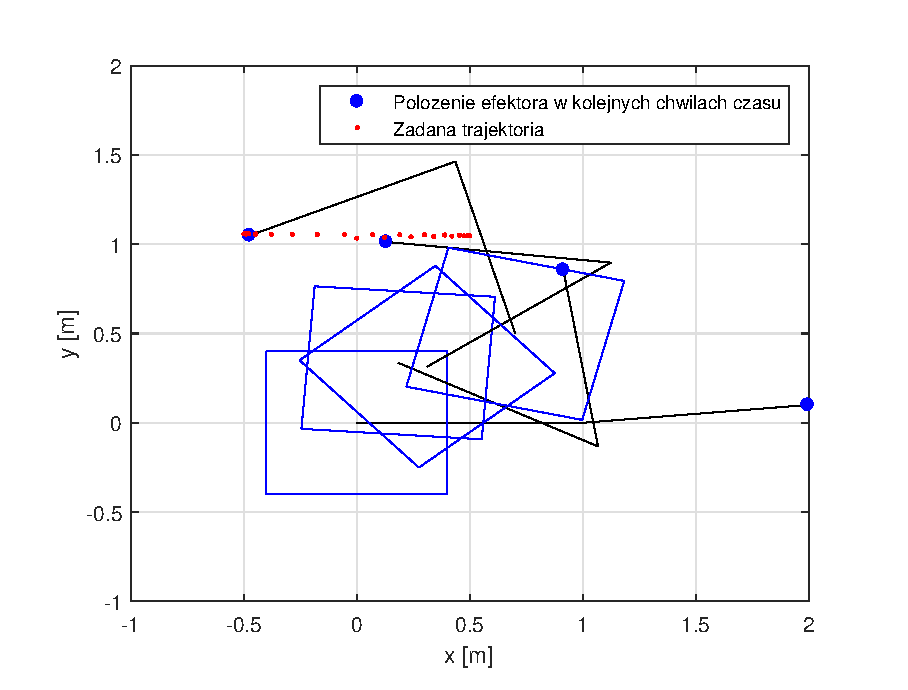
\includegraphics[width=.8\linewidth]{pics/FF1BaryDrawing}
\caption{Robot free-floating z manipulatorem w kolejnych chwilach czasu}
\label{fig:FF1Drawing}
\end{figure}

Przebiegi błędów śledzenia trajektorii chwytaka pokazano na rys. \ref{fig:FF1Barye}
\begin{figure}[H]
\centering
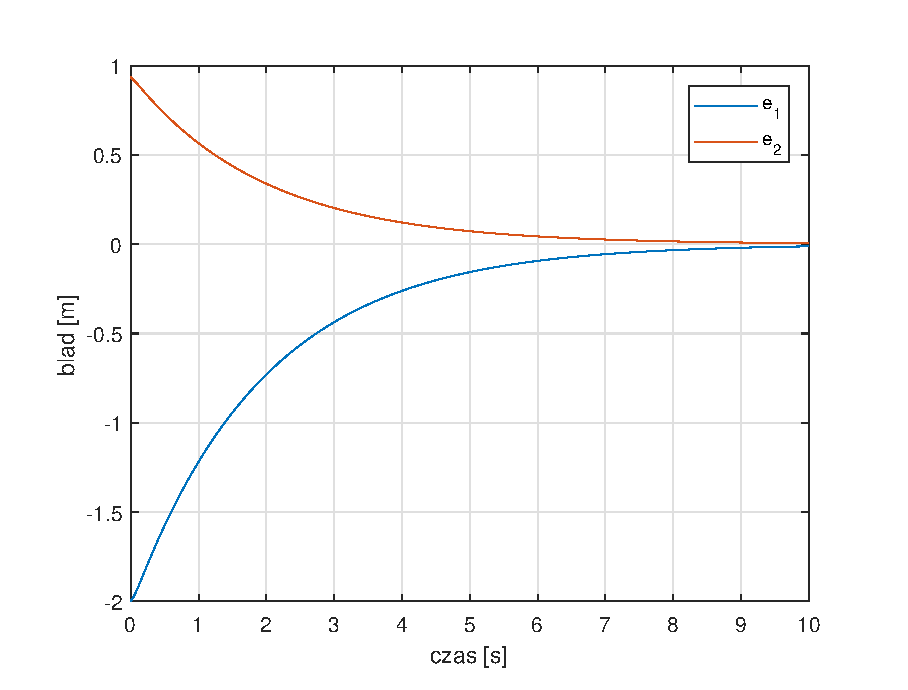
\includegraphics[width=.6\linewidth]{pics/FF1Barye}
\caption{Przebiegi błędów śledzenia trajektorii chwytaka}
\label{fig:FF1Barye}
\end{figure}

Przebiegi współrzędnych uogólnionych $q_b$ i $q_r$ pokazano na rys. \ref{fig:FF1BaryQ}
\begin{figure}[H]
\centering 
\begin{minipage}{.5\textwidth}
  	\centering
  	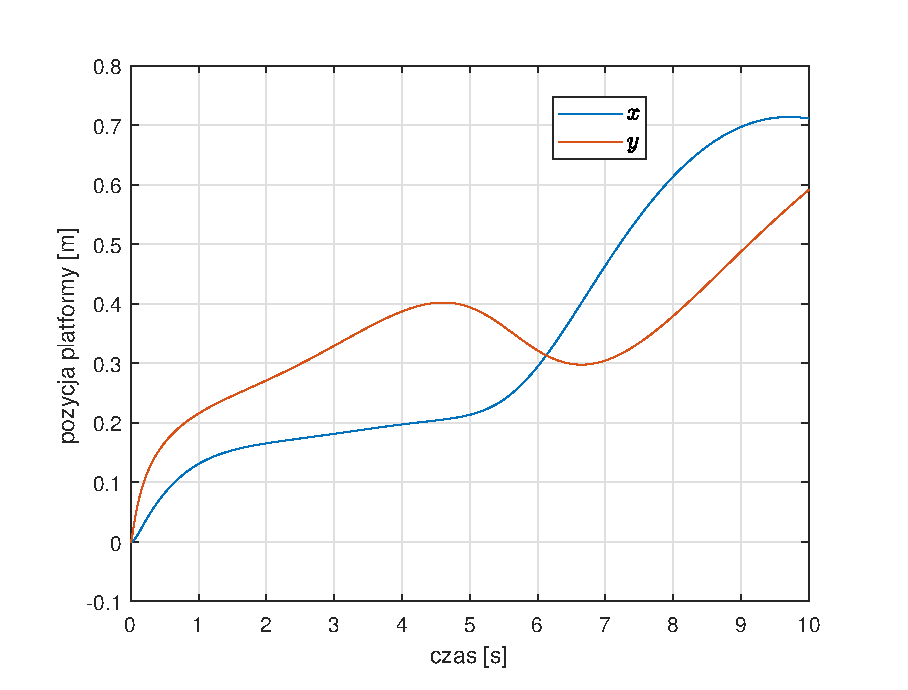
\includegraphics[width=.99\linewidth]{pics/FF1BaryX}
\end{minipage}%
\begin{minipage}{.5\textwidth}
 	\centering
    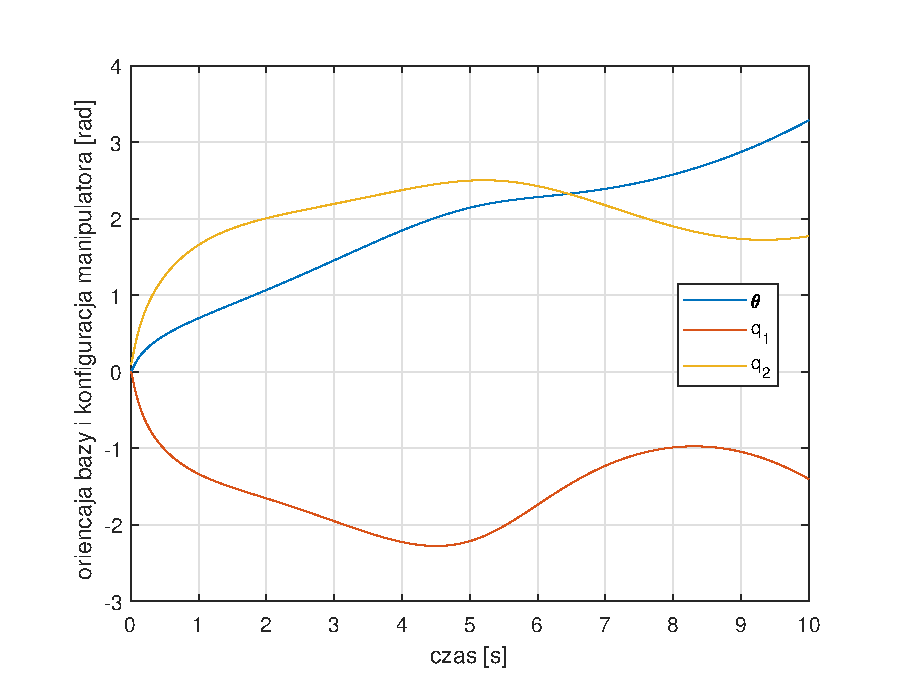
\includegraphics[width=.99\linewidth]{pics/FF1BaryQ}
\end{minipage}%
\caption{Przebiegi współrzędnych uogólnionych $q_b$ i $q_r$}
\label{fig:FF1BaryQ}
\end{figure}

Przebiegi współrzędnych barycentrycznych $\bar{x}$ i $\bar{y}$ i ich prędkości pokazano na rys. \ref{fig:FF1BaryXBAR}
\begin{figure}[H]
\centering 
\begin{minipage}{.5\textwidth}
  	\centering
  	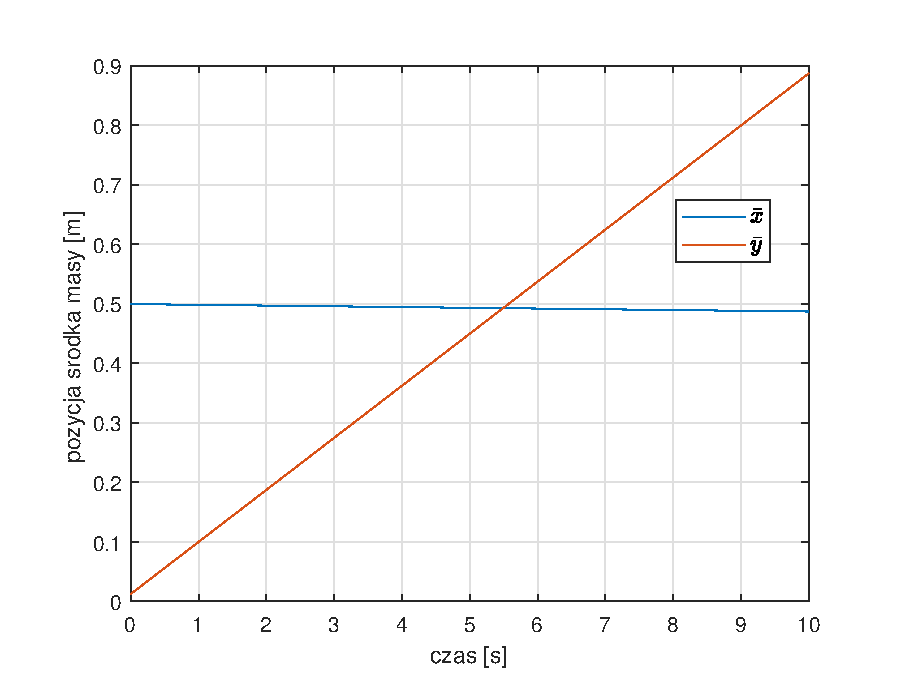
\includegraphics[width=.99\linewidth]{pics/FF1BaryXBAR}
\end{minipage}%
\begin{minipage}{.5\textwidth}
 	\centering
    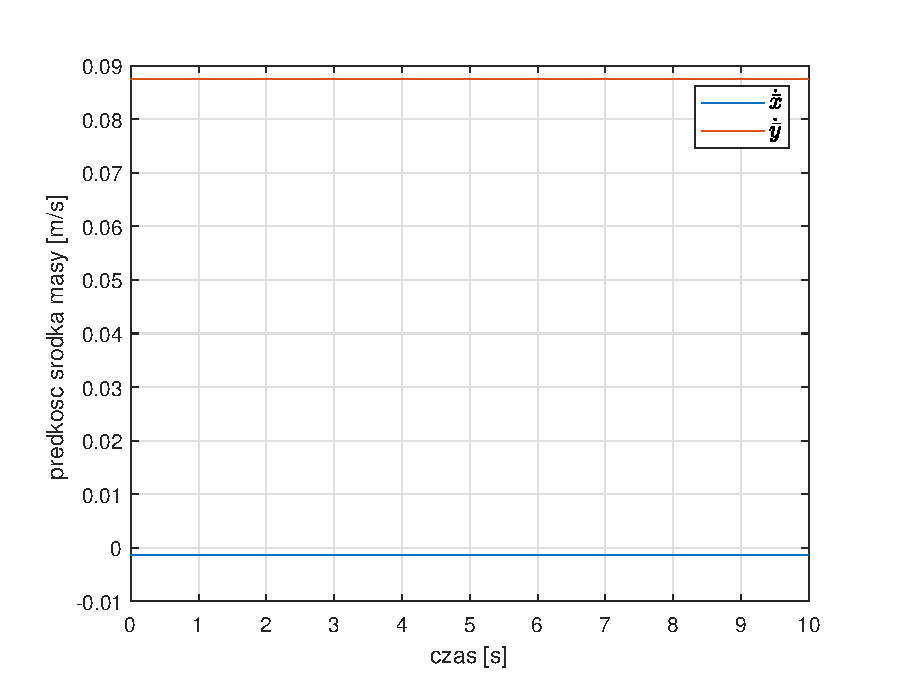
\includegraphics[width=.99\linewidth]{pics/FF1BaryXBARP}
\end{minipage}%
\caption{Przebiegi współrzędnych barycentrycznych $\bar{x}$ i $\bar{y}$ i ich prędkości}
\label{fig:FF1BaryXBAR}
\end{figure}
\begin{thebibliography}{99}
\bibitem{1} Mazur A. \textit{New approach to designing input-output decoupling controllers for mobile manipulators}. Bull. of the Polish Academy of sciences Tech. Sci. 53(1):31-37, (2005)

\bibitem{2} Yamamoto Y, Yun X. \textit{Coordinating locomotion and manipulation of a mobile manipulator.} IEEE Trans. on Automatic Control, 39(6):1326-1332, (1994)

\bibitem{3} Yamamoto Y, Yun X. \textit{Effect of the dynamic interaction on coordinated control of mobile manipulators.} IEEE Trans. Robotics Automat, 12(5):816-824, (1996)

\bibitem{4} Mazur A, Arent K. \textit{Lecture Notes in Control and Information Sciences}, 335:55-71 (2007)

\bibitem{5} Tchoń K, Jakubiak J. \textit{Acceleration-Driven Kinematics of Mobile Manipulators: An Endogenous Configuration Space Approach}, pp.(469-476),  (2004)

\bibitem{6} M. R. Flannery. \textit{The Enigma of Nonholonomic Constraints.} American Association of Physics Teachers, 73(3):265–272, (2005).

\bibitem{7} Yamamoto Y, Yun X. \textit{Coordinating locomotion and manipulation of a mobile manipulator.} In Proceedings of 31st IEEE Conference on Decision and Control, pp.(2643-2648), (1992)
\end{thebibliography}

%\addcontentsline{toc}{chapter}{Bibliografia}
\begin{thebibliography}{10}
\bibitem{AlSa16} A. Salwach, "Wizualizacja i analiza robotyczna postury bramkarza sportowego", inżynierska praca dyplomowa, Wydział
  Elektroniki, Politechnika Wrocławska 2016.  
\bibitem{Kinect} http://www.xbox.com/en-US/xbox-one/accessories/kinect
\bibitem{game} J. D. Williams, "Strateg doskonały. Wprowadzenie do teorii gier", PWN, Warszawa 1965
\bibitem{game2} http://www.fuw.edu.pl/\textasciitilde kostecki/teoria\underline{\hspace{.1in}}gier.pdf
\bibitem{MSpong} M. Spong, M. Vidyasagar, "Dynamika i sterowanie robotów", WNT, Warszawa 1997
\bibitem{Eigen} http://eigen.tuxfamily.org/
\bibitem{rapidXml} http://rapidxml.sourceforge.net/
\bibitem{doxygen} http://www.stack.nl/\textasciitilde dimitri/doxygen/
\bibitem{qt} https://www.qt.io/qt5-7/
\bibitem{body} R. Contini, "Body Segment Parametsrs, Part II", \textit{Artificial Limbs}, Washington D.C. 1972
\bibitem{Wolfram} C. Hastings, K. Mischo, M. Morrison, "Hands-On Start to Wolfram Mathematica", Wolfram Media, Inc. 2015
\bibitem{multiresgrid} R. D. Jovanović, M. Tuba, D. Simian, "An Algorithm for
  Multi-Resolution Grid Creation Applied to Explicit Finite Difference Scheme",
  Proc.\  of the 12th WSEAS Int.\ Conf.\ on COMPUTERS 2008. 
\end{thebibliography}




%\bibliography{bibliografia} % bibliografia.bib

%opcjonalnie może się tu pojawić spis rysunków i tabel
% \listoffigures
% \listoftables
\end{document}
